% figures created by /modules/module_objfn.sas
% last updated:


%\begin{figure}\centering
%\caption{Objective Function Values, 1990-2010 \label{fig:objfn_raw}}
%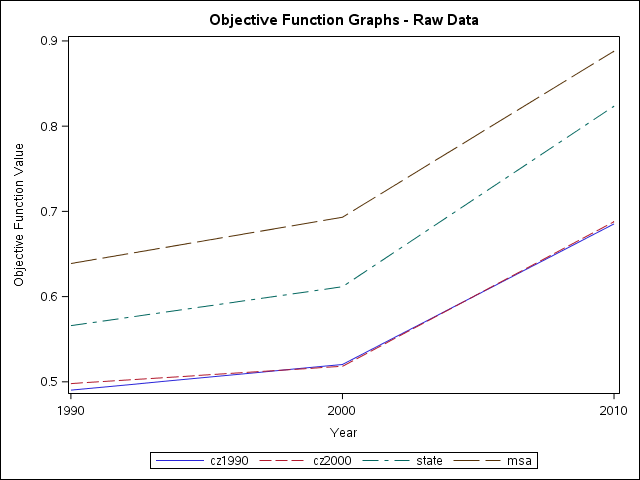
\includegraphics[scale=.6]{./figures/objectivefn_raw.png}
%\end{figure}

%\begin{figure}\centering
%\caption{Normalized Objective Function Values, 1990-2010 \label{fig:objfn_norm}}
%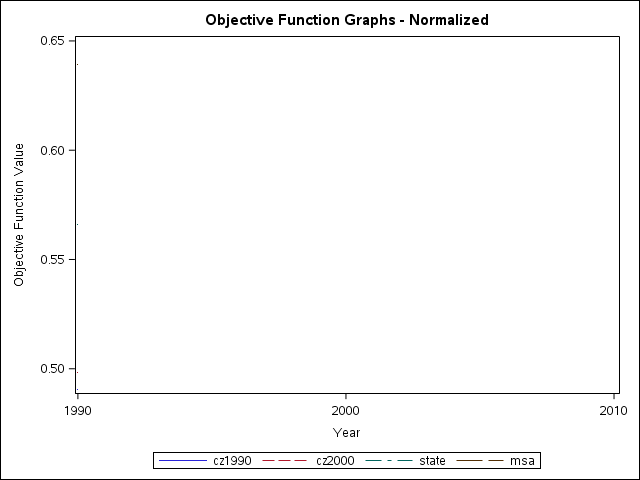
\includegraphics[scale=.5]{./figures/objectivefn_norm.png}
%\end{figure}

\begin{figure}\centering
\caption{Normalized Objective Function Values - Including Optimal Clusters, 1990-2010 \label{fig:objfn_norm_fastclus}}
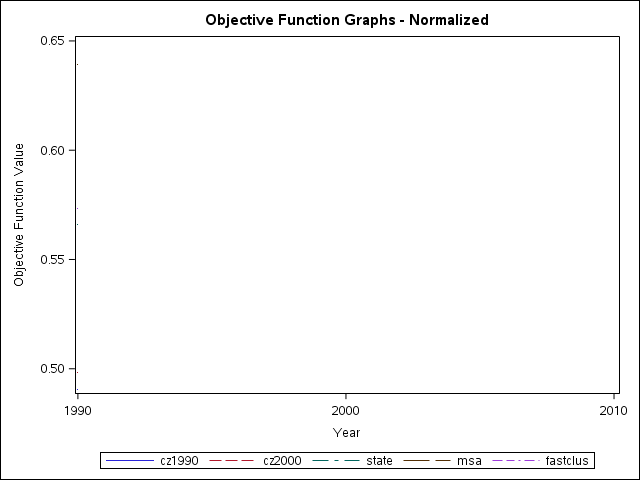
\includegraphics[scale=.5]{./figures/objectivefn_norm1.png}\\
\floatfoot{\textit{Notes}: The cluster mappings cz1990 and cz2000 refer to the definitions of 1990 and 2000 Commuting Zones. State and MSA refer to mappings of counties to States and CBSAs. Fastclus refers to the Mobility Zones mapping, based on the k-means methodology known in SAS as PROC FASTCLUS. All objective function evaluations are normalized by the evaluation of Random Zones.}
\end{figure}
